

\tikzset{every picture/.style={line width=0.95pt}} %set default line width to 0.75pt        

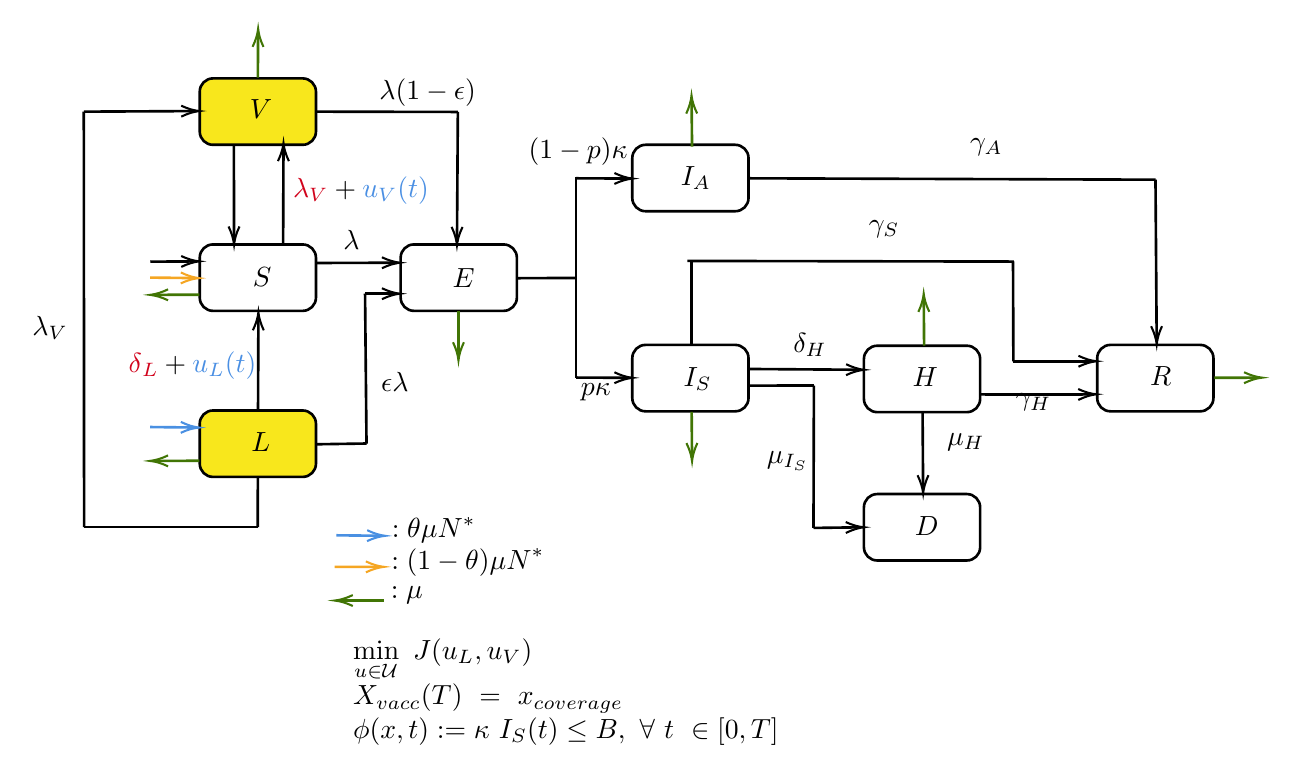
\begin{tikzpicture}[x=0.75pt,y=0.75pt,yscale=-0.8,xscale=0.8]
%uncomment if require: \path (0,472); %set diagram left start at 0, and has height of 472

%Rounded Rect [id:dp9338258576556762] 
\draw   (131,159) .. controls (131,154.58) and (134.58,151) .. (139,151) -- (193,151) .. controls (197.42,151) and (201,154.58) .. (201,159) -- (201,183) .. controls (201,187.42) and (197.42,191) .. (193,191) -- (139,191) .. controls (134.58,191) and (131,187.42) .. (131,183) -- cycle ;
%Rounded Rect [id:dp03550846434827437] 
\draw   (252,159) .. controls (252,154.58) and (255.58,151) .. (260,151) -- (314,151) .. controls (318.42,151) and (322,154.58) .. (322,159) -- (322,183) .. controls (322,187.42) and (318.42,191) .. (314,191) -- (260,191) .. controls (255.58,191) and (252,187.42) .. (252,183) -- cycle ;
%Rounded Rect [id:dp2096597210016533] 
\draw   (391.5,99) .. controls (391.5,94.58) and (395.08,91) .. (399.5,91) -- (453.5,91) .. controls (457.92,91) and (461.5,94.58) .. (461.5,99) -- (461.5,123) .. controls (461.5,127.42) and (457.92,131) .. (453.5,131) -- (399.5,131) .. controls (395.08,131) and (391.5,127.42) .. (391.5,123) -- cycle ;
%Rounded Rect [id:dp4192775592826552] 
\draw   (391.5,219.5) .. controls (391.5,215.08) and (395.08,211.5) .. (399.5,211.5) -- (453.5,211.5) .. controls (457.92,211.5) and (461.5,215.08) .. (461.5,219.5) -- (461.5,243.5) .. controls (461.5,247.92) and (457.92,251.5) .. (453.5,251.5) -- (399.5,251.5) .. controls (395.08,251.5) and (391.5,247.92) .. (391.5,243.5) -- cycle ;
%Rounded Rect [id:dp9412674774350195] 
\draw   (671.5,219.5) .. controls (671.5,215.08) and (675.08,211.5) .. (679.5,211.5) -- (733.5,211.5) .. controls (737.92,211.5) and (741.5,215.08) .. (741.5,219.5) -- (741.5,243.5) .. controls (741.5,247.92) and (737.92,251.5) .. (733.5,251.5) -- (679.5,251.5) .. controls (675.08,251.5) and (671.5,247.92) .. (671.5,243.5) -- cycle ;
%Rounded Rect [id:dp7750331540351684] 
\draw   (531,309.33) .. controls (531,304.92) and (534.58,301.33) .. (539,301.33) -- (593,301.33) .. controls (597.42,301.33) and (601,304.92) .. (601,309.33) -- (601,333.33) .. controls (601,337.75) and (597.42,341.33) .. (593,341.33) -- (539,341.33) .. controls (534.58,341.33) and (531,337.75) .. (531,333.33) -- cycle ;
%Rounded Rect [id:dp22729858034129236] 
\draw   (531,220) .. controls (531,215.58) and (534.58,212) .. (539,212) -- (593,212) .. controls (597.42,212) and (601,215.58) .. (601,220) -- (601,244) .. controls (601,248.42) and (597.42,252) .. (593,252) -- (539,252) .. controls (534.58,252) and (531,248.42) .. (531,244) -- cycle ;
%Straight Lines [id:da8056305543799926] 
\draw    (201.33,162.17) -- (249.67,162.01) ;
\draw [shift={(251.67,162)}, rotate = 539.81] [color={rgb, 255:red, 0; green, 0; blue, 0 }  ][line width=0.75]    (10.93,-3.29) .. controls (6.95,-1.4) and (3.31,-0.3) .. (0,0) .. controls (3.31,0.3) and (6.95,1.4) .. (10.93,3.29)   ;
%Straight Lines [id:da2787683579538649] 
\draw    (322.78,171.33) -- (357.67,171.17) ;
%Straight Lines [id:da21916666537860907] 
\draw    (357.67,111.17) -- (389.67,111.32) ;
\draw [shift={(391.67,111.33)}, rotate = 180.28] [color={rgb, 255:red, 0; green, 0; blue, 0 }  ][line width=0.75]    (10.93,-3.29) .. controls (6.95,-1.4) and (3.31,-0.3) .. (0,0) .. controls (3.31,0.3) and (6.95,1.4) .. (10.93,3.29)   ;
%Straight Lines [id:da8438200798129222] 
\draw    (357.67,110.6) -- (357.67,231.17) ;
%Straight Lines [id:da7337155371803761] 
\draw    (357.67,231.17) -- (389.67,231.32) ;
\draw [shift={(391.67,231.33)}, rotate = 180.28] [color={rgb, 255:red, 0; green, 0; blue, 0 }  ][line width=0.75]    (10.93,-3.29) .. controls (6.95,-1.4) and (3.31,-0.3) .. (0,0) .. controls (3.31,0.3) and (6.95,1.4) .. (10.93,3.29)   ;
%Straight Lines [id:da509274682669141] 
\draw    (461.43,226) -- (516.2,226.39) -- (529.2,226.49) ;
\draw [shift={(531.2,226.5)}, rotate = 180.41] [color={rgb, 255:red, 0; green, 0; blue, 0 }  ][line width=0.75]    (10.93,-3.29) .. controls (6.95,-1.4) and (3.31,-0.3) .. (0,0) .. controls (3.31,0.3) and (6.95,1.4) .. (10.93,3.29)   ;
%Straight Lines [id:da3183759306298827] 
\draw    (500.63,321.73) -- (529,321.36) ;
\draw [shift={(531,321.33)}, rotate = 539.25] [color={rgb, 255:red, 0; green, 0; blue, 0 }  ][line width=0.75]    (10.93,-3.29) .. controls (6.95,-1.4) and (3.31,-0.3) .. (0,0) .. controls (3.31,0.3) and (6.95,1.4) .. (10.93,3.29)   ;
%Straight Lines [id:da6861028849351065] 
\draw    (462,236) -- (500.88,235.98) ;
%Straight Lines [id:da9190171216881116] 
\draw    (500.88,235.98) -- (500.63,321.73) ;
%Straight Lines [id:da03313994658252273] 
\draw    (600.33,241.33) -- (657.2,241.39) -- (669,241.27) ;
\draw [shift={(671,241.25)}, rotate = 539.4100000000001] [color={rgb, 255:red, 0; green, 0; blue, 0 }  ][line width=0.75]    (10.93,-3.29) .. controls (6.95,-1.4) and (3.31,-0.3) .. (0,0) .. controls (3.31,0.3) and (6.95,1.4) .. (10.93,3.29)   ;
%Straight Lines [id:da6934604539767528] 
\draw    (566.33,252) -- (566.65,298.92) ;
\draw [shift={(566.67,300.92)}, rotate = 269.61] [color={rgb, 255:red, 0; green, 0; blue, 0 }  ][line width=0.75]    (10.93,-3.29) .. controls (6.95,-1.4) and (3.31,-0.3) .. (0,0) .. controls (3.31,0.3) and (6.95,1.4) .. (10.93,3.29)   ;
%Straight Lines [id:da6916456040068684] 
\draw    (461,111.17) -- (706.6,112) ;
%Straight Lines [id:da7246498566982733] 
\draw    (706.6,112) -- (707.32,209.17) ;
\draw [shift={(707.33,211.17)}, rotate = 269.58] [color={rgb, 255:red, 0; green, 0; blue, 0 }  ][line width=0.75]    (10.93,-3.29) .. controls (6.95,-1.4) and (3.31,-0.3) .. (0,0) .. controls (3.31,0.3) and (6.95,1.4) .. (10.93,3.29)   ;
%Straight Lines [id:da5396778112959429] 
\draw    (427,161.17) -- (427,211.5) ;
%Straight Lines [id:da7180507787496266] 
\draw    (424.7,160.93) -- (621.3,161.32) ;
%Straight Lines [id:da3365589163505732] 
\draw    (621,221.35) -- (669.13,221.35) ;
\draw [shift={(671.13,221.35)}, rotate = 180] [color={rgb, 255:red, 0; green, 0; blue, 0 }  ][line width=0.75]    (10.93,-3.29) .. controls (6.95,-1.4) and (3.31,-0.3) .. (0,0) .. controls (3.31,0.3) and (6.95,1.4) .. (10.93,3.29)   ;
%Straight Lines [id:da7818385183529692] 
\draw    (620.8,161.2) -- (621,221.35) ;
%Straight Lines [id:da20994732667721105] 
\draw [color={rgb, 255:red, 245; green, 166; blue, 35 }  ,draw opacity=1 ][fill={rgb, 255:red, 65; green, 117; blue, 5 }  ,fill opacity=1 ]   (101.15,170.97) -- (128.54,171.26) ;
\draw [shift={(130.54,171.28)}, rotate = 180.6] [color={rgb, 255:red, 245; green, 166; blue, 35 }  ,draw opacity=1 ][line width=0.75]    (10.93,-3.29) .. controls (6.95,-1.4) and (3.31,-0.3) .. (0,0) .. controls (3.31,0.3) and (6.95,1.4) .. (10.93,3.29)   ;
%Straight Lines [id:da9409632697808414] 
\draw [color={rgb, 255:red, 65; green, 117; blue, 5 }  ,draw opacity=1 ]   (130.75,181.29) -- (103,181.36) ;
\draw [shift={(101,181.37)}, rotate = 359.86] [color={rgb, 255:red, 65; green, 117; blue, 5 }  ,draw opacity=1 ][line width=0.75]    (10.93,-3.29) .. controls (6.95,-1.4) and (3.31,-0.3) .. (0,0) .. controls (3.31,0.3) and (6.95,1.4) .. (10.93,3.29)   ;
%Straight Lines [id:da671739616587531] 
\draw [color={rgb, 255:red, 65; green, 117; blue, 5 }  ,draw opacity=1 ]   (286.82,190.79) -- (286.82,218.85) ;
\draw [shift={(286.82,220.85)}, rotate = 270] [color={rgb, 255:red, 65; green, 117; blue, 5 }  ,draw opacity=1 ][line width=0.75]    (10.93,-3.29) .. controls (6.95,-1.4) and (3.31,-0.3) .. (0,0) .. controls (3.31,0.3) and (6.95,1.4) .. (10.93,3.29)   ;
%Straight Lines [id:da4612478738976049] 
\draw [color={rgb, 255:red, 65; green, 117; blue, 5 }  ,draw opacity=1 ]   (427.25,251.79) -- (427.48,279.54) ;
\draw [shift={(427.5,281.54)}, rotate = 269.52] [color={rgb, 255:red, 65; green, 117; blue, 5 }  ,draw opacity=1 ][line width=0.75]    (10.93,-3.29) .. controls (6.95,-1.4) and (3.31,-0.3) .. (0,0) .. controls (3.31,0.3) and (6.95,1.4) .. (10.93,3.29)   ;
%Straight Lines [id:da6463966696699537] 
\draw [color={rgb, 255:red, 65; green, 117; blue, 5 }  ,draw opacity=1 ]   (427.5,92.04) -- (427.19,63.25) ;
\draw [shift={(427.17,61.25)}, rotate = 449.38] [color={rgb, 255:red, 65; green, 117; blue, 5 }  ,draw opacity=1 ][line width=0.75]    (10.93,-3.29) .. controls (6.95,-1.4) and (3.31,-0.3) .. (0,0) .. controls (3.31,0.3) and (6.95,1.4) .. (10.93,3.29)   ;
%Straight Lines [id:da5390055225547872] 
\draw [color={rgb, 255:red, 65; green, 117; blue, 5 }  ,draw opacity=1 ]   (567.25,211.92) -- (567.02,182.67) ;
\draw [shift={(567,180.67)}, rotate = 449.54] [color={rgb, 255:red, 65; green, 117; blue, 5 }  ,draw opacity=1 ][line width=0.75]    (10.93,-3.29) .. controls (6.95,-1.4) and (3.31,-0.3) .. (0,0) .. controls (3.31,0.3) and (6.95,1.4) .. (10.93,3.29)   ;
%Straight Lines [id:da5965287355289506] 
\draw [color={rgb, 255:red, 65; green, 117; blue, 5 }  ,draw opacity=1 ]   (742,231.29) -- (768.88,231.23) ;
\draw [shift={(770.88,231.23)}, rotate = 539.88] [color={rgb, 255:red, 65; green, 117; blue, 5 }  ,draw opacity=1 ][line width=0.75]    (10.93,-3.29) .. controls (6.95,-1.4) and (3.31,-0.3) .. (0,0) .. controls (3.31,0.3) and (6.95,1.4) .. (10.93,3.29)   ;
%Straight Lines [id:da8186275398290976] 
\draw [color={rgb, 255:red, 245; green, 166; blue, 35 }  ,draw opacity=1 ]   (212.25,345.21) -- (240,345.17) ;
\draw [shift={(242,345.17)}, rotate = 539.9200000000001] [color={rgb, 255:red, 245; green, 166; blue, 35 }  ,draw opacity=1 ][line width=0.75]    (10.93,-3.29) .. controls (6.95,-1.4) and (3.31,-0.3) .. (0,0) .. controls (3.31,0.3) and (6.95,1.4) .. (10.93,3.29)   ;
%Straight Lines [id:da2473783506649132] 
\draw [color={rgb, 255:red, 65; green, 117; blue, 5 }  ,draw opacity=1 ]   (241.75,365.46) -- (214.25,365.46) ;
\draw [shift={(212.25,365.46)}, rotate = 360] [color={rgb, 255:red, 65; green, 117; blue, 5 }  ,draw opacity=1 ][line width=0.75]    (10.93,-3.29) .. controls (6.95,-1.4) and (3.31,-0.3) .. (0,0) .. controls (3.31,0.3) and (6.95,1.4) .. (10.93,3.29)   ;
%Rounded Rect [id:dp8809691932687975] 
\draw  [fill={rgb, 255:red, 248; green, 231; blue, 28 }  ,fill opacity=1 ] (131,259) .. controls (131,254.58) and (134.58,251) .. (139,251) -- (193,251) .. controls (197.42,251) and (201,254.58) .. (201,259) -- (201,283) .. controls (201,287.42) and (197.42,291) .. (193,291) -- (139,291) .. controls (134.58,291) and (131,287.42) .. (131,283) -- cycle ;
%Rounded Rect [id:dp20452328105731965] 
\draw  [fill={rgb, 255:red, 248; green, 231; blue, 28 }  ,fill opacity=1 ] (131,59) .. controls (131,54.58) and (134.58,51) .. (139,51) -- (193,51) .. controls (197.42,51) and (201,54.58) .. (201,59) -- (201,83) .. controls (201,87.42) and (197.42,91) .. (193,91) -- (139,91) .. controls (134.58,91) and (131,87.42) .. (131,83) -- cycle ;
%Straight Lines [id:da7332016409842015] 
\draw    (230.56,180.67) -- (249.67,180.67) ;
\draw [shift={(251.67,180.67)}, rotate = 180] [color={rgb, 255:red, 0; green, 0; blue, 0 }  ][line width=0.75]    (10.93,-3.29) .. controls (6.95,-1.4) and (3.31,-0.3) .. (0,0) .. controls (3.31,0.3) and (6.95,1.4) .. (10.93,3.29)   ;
%Straight Lines [id:da9863388911939545] 
\draw    (230.56,180.67) -- (231.44,270.89) ;
%Straight Lines [id:da8080535215203265] 
\draw    (201.25,271.35) -- (231.44,270.89) ;
%Straight Lines [id:da40743845785244703] 
\draw    (166.11,250.89) -- (166.33,193.78) ;
\draw [shift={(166.33,191.78)}, rotate = 450.22] [color={rgb, 255:red, 0; green, 0; blue, 0 }  ][line width=0.75]    (10.93,-3.29) .. controls (6.95,-1.4) and (3.31,-0.3) .. (0,0) .. controls (3.31,0.3) and (6.95,1.4) .. (10.93,3.29)   ;
%Straight Lines [id:da9322929691633284] 
\draw    (101.2,161.37) -- (128.78,161.21) ;
\draw [shift={(130.78,161.19)}, rotate = 539.6700000000001] [color={rgb, 255:red, 0; green, 0; blue, 0 }  ][line width=0.75]    (10.93,-3.29) .. controls (6.95,-1.4) and (3.31,-0.3) .. (0,0) .. controls (3.31,0.3) and (6.95,1.4) .. (10.93,3.29)   ;
%Straight Lines [id:da39718296722033697] 
\draw    (181.22,151) -- (181.44,91.89) ;
\draw [shift={(181.44,89.89)}, rotate = 450.21] [color={rgb, 255:red, 0; green, 0; blue, 0 }  ][line width=0.75]    (10.93,-3.29) .. controls (6.95,-1.4) and (3.31,-0.3) .. (0,0) .. controls (3.31,0.3) and (6.95,1.4) .. (10.93,3.29)   ;
%Straight Lines [id:da5809696066442677] 
\draw    (151.56,90.89) -- (151.66,149.11) ;
\draw [shift={(151.67,151.11)}, rotate = 269.89] [color={rgb, 255:red, 0; green, 0; blue, 0 }  ][line width=0.75]    (10.93,-3.29) .. controls (6.95,-1.4) and (3.31,-0.3) .. (0,0) .. controls (3.31,0.3) and (6.95,1.4) .. (10.93,3.29)   ;
%Straight Lines [id:da793642305015831] 
\draw [color={rgb, 255:red, 65; green, 117; blue, 5 }  ,draw opacity=1 ]   (166,50.54) -- (166.16,23.08) ;
\draw [shift={(166.17,21.08)}, rotate = 450.32] [color={rgb, 255:red, 65; green, 117; blue, 5 }  ,draw opacity=1 ][line width=0.75]    (10.93,-3.29) .. controls (6.95,-1.4) and (3.31,-0.3) .. (0,0) .. controls (3.31,0.3) and (6.95,1.4) .. (10.93,3.29)   ;
%Straight Lines [id:da6558914162483227] 
\draw    (61.18,71.03) -- (128.8,70.68) ;
\draw [shift={(130.8,70.67)}, rotate = 539.7] [color={rgb, 255:red, 0; green, 0; blue, 0 }  ][line width=0.75]    (10.93,-3.29) .. controls (6.95,-1.4) and (3.31,-0.3) .. (0,0) .. controls (3.31,0.3) and (6.95,1.4) .. (10.93,3.29)   ;
%Straight Lines [id:da352457903437118] 
\draw    (61.18,71.03) -- (61.36,321.21) ;
%Straight Lines [id:da6614557049237877] 
\draw    (166,291.3) -- (165.91,321.21) ;
%Straight Lines [id:da33095535888136296] 
\draw    (61.36,321.21) -- (165.91,321.21) ;
%Straight Lines [id:da269007580963348] 
\draw    (201.64,71.03) -- (286.45,71.21) ;
%Straight Lines [id:da3843881794607171] 
\draw    (286.45,71.21) -- (285.92,149.39) ;
\draw [shift={(285.91,151.39)}, rotate = 270.39] [color={rgb, 255:red, 0; green, 0; blue, 0 }  ][line width=0.75]    (10.93,-3.29) .. controls (6.95,-1.4) and (3.31,-0.3) .. (0,0) .. controls (3.31,0.3) and (6.95,1.4) .. (10.93,3.29)   ;
%Straight Lines [id:da5569228544903815] 
\draw [color={rgb, 255:red, 74; green, 144; blue, 226 }  ,draw opacity=1 ][fill={rgb, 255:red, 65; green, 117; blue, 5 }  ,fill opacity=1 ]   (101.15,260.97) -- (128.54,261.26) ;
\draw [shift={(130.54,261.28)}, rotate = 180.6] [color={rgb, 255:red, 74; green, 144; blue, 226 }  ,draw opacity=1 ][line width=0.75]    (10.93,-3.29) .. controls (6.95,-1.4) and (3.31,-0.3) .. (0,0) .. controls (3.31,0.3) and (6.95,1.4) .. (10.93,3.29)   ;
%Straight Lines [id:da8309131427834217] 
\draw [color={rgb, 255:red, 65; green, 117; blue, 5 }  ,draw opacity=1 ]   (130.75,281.29) -- (103,281.36) ;
\draw [shift={(101,281.37)}, rotate = 359.86] [color={rgb, 255:red, 65; green, 117; blue, 5 }  ,draw opacity=1 ][line width=0.75]    (10.93,-3.29) .. controls (6.95,-1.4) and (3.31,-0.3) .. (0,0) .. controls (3.31,0.3) and (6.95,1.4) .. (10.93,3.29)   ;
%Straight Lines [id:da0682900101015288] 
\draw [color={rgb, 255:red, 74; green, 144; blue, 226 }  ,draw opacity=1 ][fill={rgb, 255:red, 65; green, 117; blue, 5 }  ,fill opacity=1 ]   (213.35,326.17) -- (240.74,326.46) ;
\draw [shift={(242.74,326.48)}, rotate = 180.6] [color={rgb, 255:red, 74; green, 144; blue, 226 }  ,draw opacity=1 ][line width=0.75]    (10.93,-3.29) .. controls (6.95,-1.4) and (3.31,-0.3) .. (0,0) .. controls (3.31,0.3) and (6.95,1.4) .. (10.93,3.29)   ;

% Text Node
\draw (161,163) node [anchor=north west][inner sep=0.75pt]   [align=left] {$\displaystyle S$};
% Text Node
\draw (281.33,163.33) node [anchor=north west][inner sep=0.75pt]   [align=left] {$\displaystyle E$};
% Text Node
\draw (418.67,102) node [anchor=north west][inner sep=0.75pt]   [align=left] {$\displaystyle I_{A}$};
% Text Node
\draw (420.33,223.33) node [anchor=north west][inner sep=0.75pt]   [align=left] {$\displaystyle I_{S}$};
% Text Node
\draw (558.33,223) node [anchor=north west][inner sep=0.75pt]   [align=left] {$\displaystyle H$};
% Text Node
\draw (701.33,222.33) node [anchor=north west][inner sep=0.75pt]   [align=left] {$\displaystyle R$};
% Text Node
\draw (559.67,312.67) node [anchor=north west][inner sep=0.75pt]   [align=left] {$\displaystyle D$};
% Text Node
\draw (244,355.17) node [anchor=north west][inner sep=0.75pt]   [align=left] {$\displaystyle :\mu $};
% Text Node
\draw (244.33,332) node [anchor=north west][inner sep=0.75pt]   [align=left] {$\displaystyle :( 1-\theta ) \mu N^{*}$};
% Text Node
\draw (215.5,140.67) node [anchor=north west][inner sep=0.75pt]   [align=left] {$\displaystyle \lambda $};
% Text Node
\draw (358.5,232.5) node [anchor=north west][inner sep=0.75pt]   [align=left] {$\displaystyle p\kappa $};
% Text Node
\draw (327,85) node [anchor=north west][inner sep=0.75pt]   [align=left] {$\displaystyle ( 1-p) \kappa $};
% Text Node
\draw (593,85) node [anchor=north west][inner sep=0.75pt]   [align=left] {$\displaystyle \gamma _{A}$};
% Text Node
\draw (532,134.5) node [anchor=north west][inner sep=0.75pt]   [align=left] {$\displaystyle \gamma _{S}$};
% Text Node
\draw (486.5,202.5) node [anchor=north west][inner sep=0.75pt]   [align=left] {$\displaystyle \delta _{H}$};
% Text Node
\draw (579,263) node [anchor=north west][inner sep=0.75pt]   [align=left] {$\displaystyle \mu _{H}$};
% Text Node
\draw (620.5,239) node [anchor=north west][inner sep=0.75pt]   [align=left] {$ $$\displaystyle \gamma _{H}$};
% Text Node
\draw (470.5,273.5) node [anchor=north west][inner sep=0.75pt]   [align=left] {$\displaystyle \mu _{I_{S}}$};
% Text Node
\draw (160,262) node [anchor=north west][inner sep=0.75pt]   [align=left] {$\displaystyle L$};
% Text Node
\draw (159.2,62) node [anchor=north west][inner sep=0.75pt]   [align=left] {$\displaystyle V$};
% Text Node
\draw (185.17,108) node [anchor=north west][inner sep=0.75pt]   [align=left] {$\displaystyle \textcolor[rgb]{0.82,0.01,0.11}{\lambda }\textcolor[rgb]{0.82,0.01,0.11}{_{V}} +\textcolor[rgb]{0.29,0.56,0.89}{u}\textcolor[rgb]{0.29,0.56,0.89}{_{V}}\textcolor[rgb]{0.29,0.56,0.89}{(}\textcolor[rgb]{0.29,0.56,0.89}{t}\textcolor[rgb]{0.29,0.56,0.89}{)}$};
% Text Node
\draw (86.17,213.33) node [anchor=north west][inner sep=0.75pt]   [align=left] {$\displaystyle \textcolor[rgb]{0.82,0.01,0.11}{\delta }\textcolor[rgb]{0.82,0.01,0.11}{_{L}} +\textcolor[rgb]{0.29,0.56,0.89}{u}\textcolor[rgb]{0.29,0.56,0.89}{_{L}}\textcolor[rgb]{0.29,0.56,0.89}{(}\textcolor[rgb]{0.29,0.56,0.89}{t}\textcolor[rgb]{0.29,0.56,0.89}{)}$};
% Text Node
\draw (28.17,192) node [anchor=north west][inner sep=0.75pt]   [align=left] {$\displaystyle \textcolor[rgb]{0,0,0}{\lambda }\textcolor[rgb]{0,0,0}{_{V}}$};
% Text Node
\draw (237.17,49) node [anchor=north west][inner sep=0.75pt]   [align=left] {$\displaystyle \textcolor[rgb]{0,0,0}{\lambda }\textcolor[rgb]{0,0,0}{(}\textcolor[rgb]{0,0,0}{1-\epsilon }\textcolor[rgb]{0,0,0}{)}$};
% Text Node
\draw (238.17,226) node [anchor=north west][inner sep=0.75pt]   [align=left] {$\displaystyle \textcolor[rgb]{0,0,0}{\epsilon \lambda }$};
% Text Node
\draw (213,385) node [anchor=north west][inner sep=0.75pt]   [align=left] {$\displaystyle  \begin{array}{{>{\displaystyle}l}}
\min_{u\in \mathcal{U}} \ J( u_{L} ,u_{V})\\
X_{vacc}( T) \ =\ x_{coverage}\\
\phi ( x,t) :=\kappa \ I_{S}( t) \leq B,\ \forall \ t\ \in [ 0,T]
\end{array}$};
% Text Node
\draw (244.6,313.27) node [anchor=north west][inner sep=0.75pt]   [align=left] {$\displaystyle :\theta \mu N^{*}$};


\end{tikzpicture}
